\chapter{Simulation}

Monte Carlo simulation was used for both validation of the event selection algorithms
and determination of the energy cut efficiencies and uncertainty.
Two independent simulation programs were developed to achieve these goals.

\section{Event Selection Monte Carlo}
\label{sec:toymc}

A Monte Carlo simulation was developed to model the time correlation structure
of the Daya Bay data stream \cite{dyb_toymc, dyb_toymc_docdb}.
The simulation uses placeholder values for most quantities such as reconstructed energy
rather than simulating particle trajectories and interactions in the LS and PMTs,
hence it is known as a ``toy Monte Carlo.''
The internal details and basic functionality of the simulation,
as well as a sample of the validation studies that used simulated data,
will be described.

The simulation is based on a collection of event types:
Single, Correlated, and Muon.
Additional event types can be added if additional functionality is desired.
The simulation's configuration allows for customization of the event rate
for each different event type,
and also for multiple variants of the event type.
For example, one type of Correlated event could be configured to represent nH IBDs,
and a second type could be configured to represent nGd IBDs
with a shorter coincidence time, higher delayed energy,
and with the delayed event position limited to the GdLS (IAV) region of the AD.
%Crucially, since the prompt and delayed events are correlated,
%they are generated together by the simulation,
%so the rate of Correlated events is the rate of prompt-delayed pairs;
%similarly, for Muon events, the rate represents the rate of physical muons
%rather than the sum of rates of muon-like signals in the water pools and ADs.
When the simulation is executed,
the appropriate number of each type of event is generated
based on the desired time interval to be simulated.
The events are then time-ordered
and saved to disk in the same ROOT file data format
as produced by the Daya Bay data production.
An additional ROOT TTree structure containing the ``truth information''
for each event is included in the output data file.
For this simulation, the only ``truth'' hidden from the data output
is the event type that the given data entry represents.
The characteristics associtated with the different event types
are described below.

Single events represent uncorrelated signals,
which in Daya Bay are mostly due to natural radioactive decays in the AD
(\cref{subsec:singles}).
In the simulation, Single events are assigned timestamps
drawn uniformly at random between the time limits given in the configuration,
representing their uncorrelated nature.
The event energies are also drawn uniformly at random
between \SIlist{1;3.5}{\MeV},
and the positions are similarly randomly assigned
within the OAV cylinder.

Correlated events represent pairs of signals
with a common physical origin, both in position and in time.
IBDs and correlated backgrounds (\cref{sec:correlated_bg})
satisfy these criteria for being modeled by the Correlated event type.
To create the time correlation between prompt and delayed events,
modeled as an exponential distribution,
the simulation first determines the timestamp for a prompt event at random.
Then the coincidence time delay between prompt and delayed events is generated
from an exponential distribution
whose scale is specified in the simulation configuration.
The prompt and delayed energies are determined independently at random
using uniform distributions specified by the simulation configuration.
The position of the prompt event is chosen at random
within the GdLS or LS volumes (again, as specified by the configuration),
and the delayed position is chosen to be correlated with the prompt position.
Since exact modeling of the position correlations is not crucial,
a simple exponential distribution is used to determine the displacement
in each direction ($x,y,$ and $z$).

Muon events represent signals created by muons traversing
the water pools and ADs (\cref{sec:muonveto}).
For simplicity, each muon is assumed to create a signal
in the inner water pool with probability \num{1}.
A portion of the muon signals, by default \SI{19.95}{\percent},
traverse the AD, depositing an energy chosen at random between
\SIlist{20;2000}{\MeV}.
A smaller subset of the muon signals, by default \SI{0.05}{\percent},
creat particle showers in the AD, depositing an energy chosen at random between
\SIlist{2500;5000}{\MeV}.
These fractions and energies were chosen as defaults to approximately model
the true distributions and rates of muon signals in the near halls (EH1 and EH2).
The time delay between WP and AD muons is assigned to be \SI{50}{\ns},
chosen since in real data there a nonzero time offset between WP and AD muons,
but the distribution of time offsets
is not a critical feature of the event selection.

\subsection{Uncorrelated event rate}

The procedure for determining the uncorrelated event rate
is described in \cref{subsec:singles}.
This process, both the abstract procedure and the actual software implementation,
was validated using simulated datasets.
The simulation was configured to generate Single (uncorrelated) events
with a rate of \SI{20}{\Hz}
in data files also containing Muon and Correlated events.
The full configuration is listed in \cref{tab:toymc_singles_config}.
The simulation was used to generate 100 data sets,
each consisting of 300 files containing 10 minutes' worth of data,
for a total of 50 hours of data per data set.
The data files were processed using the event selection software
and an empirical rate for uncorrelated events was extracted
for each of the 100 data sets.
The distribution of measured uncorrelated event rates
is shown in \cref{fig:toymc_singles_dist}.
The mean singles rate was \SI{19.9935}{\Hz},
which is a bias of \SI{0.033}{\percent} relative to the ``true'' input rate.

It was hypothesized that the bias was due to an unintended effect
of the absolute fixed input event rate,
which does not fluctuate according to Poisson statistics in the simulation.
Each simulated 10-minute data file has precisely the same number of uncorrelated events,
which violates the assumption that the number of events follows the Poisson distribution.
If individual data files were longer, then any impact on the measured singles rate
should be suppressed.
A second set of 100 data sets was generated to test this hypothesis,
where each data set was a single 1000-minute data file.
The distributrion of measured uncorrelated event rates from this second data set
is shown in \cref{fig:toymc_singles_dist}.
There was a larger spread due to the shorter duration of each data file,
but the mean over all 100 data sets was \SI{19.9966}{\Hz},
which is a bias of \SI{0.017}{\percent}.
The bias decreased as the length of the simulated data file increased
(even as the number of events in the data set decreased),
validating both the origin of the bias
and that the event selection software can successfully extract
the uncorrelated event rate with minimal bias.

\begin{table}[ht]
    \centering
    \begin{tabular}[t]{llll}
        \hline
        Event type & {Rate [\si{\Hz}]} & Energy [\si{\MeV}] & Coincidence time [\si{\us}]\\
        \hline
        Single & \num{20} & $[\num{1.5}, \num{3}]$ & -\\
        \multirow{2}{*}{Correlated (nH)}
               & \multirow{2}{*}{\num{0.005}}
               & [\num{0.7}, \num{4}] (prompt)
               & \multirow{2}{*}{\num{150}} \\
               & & [\num{1.9}, \num{2.3}] (delayed) & \\
        \multirow{2}{*}{Correlated (nGd)}
               & \multirow{2}{*}{\num{0.0067}}
               & [\num{0.7}, \num{4}] (prompt)
               & \multirow{2}{*}{\num{28}} \\
               & & [\num{7}, \num{9}] (delayed) & \\
        Water Pool Muon & \num{200} & - & - \\
        AD Muon & \num{39.9} & [\num{20}, \num{2000}] & -\\
        Showering Muon & \num{0.1} & [\num{2500}, \num{5000}] & -\\
    \end{tabular}
    \caption{Simulation configuration inputs for the uncorrelated event rate study.}
    \label{tab:toymc_singles_config}
\end{table}

\begin{figure}
    \centering
    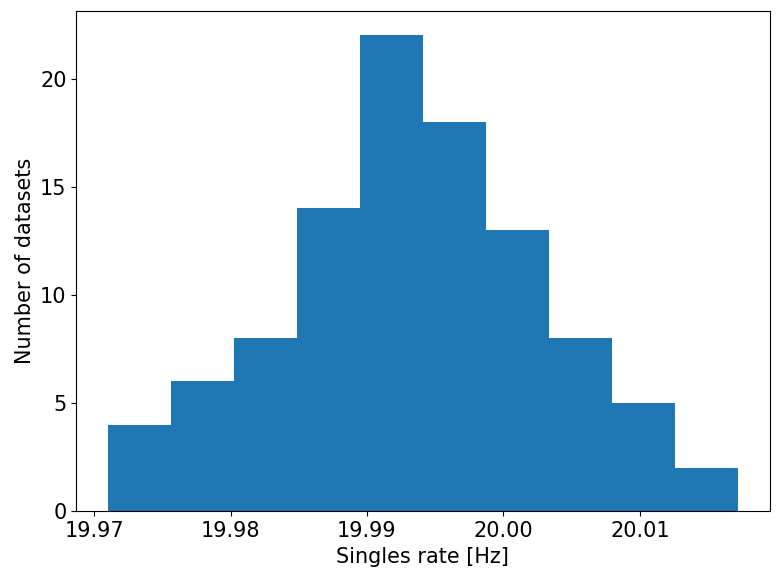
\includegraphics[width=0.7\textwidth]{ch_simulation/singles_rate_dist}
    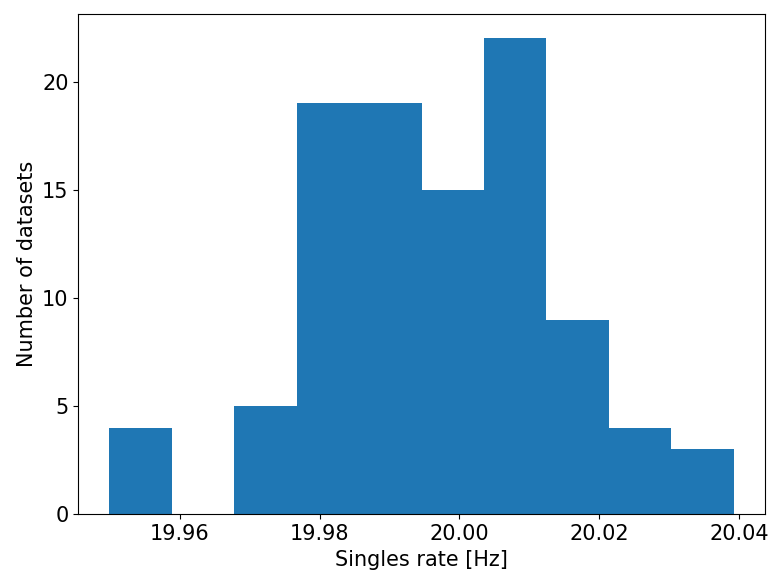
\includegraphics[width=0.7\textwidth]{ch_simulation/singles_rate_unbiased_dist}
    \caption{
        Distribution of uncorrelated event rates over 100 simulated data sets.
        The simulation configuration (``truth'') specified a rate of \SI{20}{\Hz}.
        Top: Each data set consists of 300 data files, each with 10 minutes of data.
        Bottom: Each data set consists of a single 1000-minute data file.
    }
    \label{fig:toymc_singles_dist}
\end{figure}

\subsection{Muon-induced isotopes}
\label{subsec:toymc_li9}

The Muon event type was augmented to provide validation
of the software used to search for decays of muon-induced isotopes
(\cref{subsec:li9}).
In addition to generating water pool, AD and showering muons,
the simulation also generated muon-correlated neutrons
and muon-correlated unstable isotope decays
meant to represent \li and \he.
The analysis software identified a muon as neutron-tagged
if it was followed by a neutron-like signal
with a delay of between \SIlist{20;200}{\us}.
Since the truth labels recorded whether a muon signal
was accompanied by a neutron tag,
the list of neutron-tagged muons found by the analysis software
could be compared with the list of ``true'' neutron-tagged muons
to validate the functionality of the neutron tagger.
\todo[inline]{Update when Li-9 analysis is more mature}

\subsection{Flashers}
\label{subsec:toymc_flashers}

Light emission by PMTs caused a background of single events
known as flashers (\cref{sec:flashers}).
The vast majority of flasher events are rejected using an event-by-event veto,
and the remaining flashers are assumed to be accounted for
by the treatment of the accidental background (\cref{sec:acc}).
Certain PMTs were observed to flash with a characteristic period of $\sim$ \SI{1}{\s},
which breaks the assumption in the accidental background analysis
that all single events are uncorrelated and governed by Poisson statistics.
A Flasher event type was added to the simulation to test the impact of this deviation.

The Flasher event type had a fixed energy
and generated events were given fixed, deterministic timestamps \SI{1}{\s} apart.
A data sample was generated with only Single events and Flasher events,
and was treated as if the Flasher events passed the existing flasher veto criteria.
The accidental background analysis was performed on this data sample,
with the expected output of \num{0} coincident events remaining
after subtracting the accidental background.
However, the actual output number of events was negative.
Further inspection showed that the residual flasher events,
like all other single events,
contributed to the synthetic accidentals sample,
and in that sample some of the pairs
were composed of two residual flasher events.
In the real (simulated) data set, though,
there were no accidental coincidences between residual flashers by construction,
since the residual flasher events were generated with \SI{1}{\s} time gaps
between consecutive flashers.
\todo[inline]{Add more when Olivia reports back}

\section{Efficiency Monte Carlo}
\label{sec:thu_toymc}
